%-------------------------
% Resume in Latex
% Author
% License : MIT
%------------------------

%---- Required Packages and Functions ----

\documentclass[a4paper,11pt]{article}
\usepackage{latexsym}
\usepackage{xcolor}
\usepackage{float}
\usepackage{ragged2e}
\usepackage[empty]{fullpage}
\usepackage{wrapfig}
\usepackage{lipsum}
\usepackage{tabularx}
\usepackage{titlesec}
\usepackage{geometry}
\usepackage{marvosym}
\usepackage{verbatim}
\usepackage{enumitem}
\usepackage[hidelinks]{hyperref}
\usepackage{fancyhdr}
\usepackage{fontawesome5}
\usepackage{multicol}
\usepackage{graphicx}
\usepackage{cfr-lm}
\usepackage[T1]{fontenc}
\setlength{\multicolsep}{0pt} 
\pagestyle{fancy}
\fancyhf{} % clear all header and footer fields
\fancyfoot{}
\renewcommand{\headrulewidth}{0pt}
\renewcommand{\footrulewidth}{0pt}
\geometry{left=1.4cm, top=0.8cm, right=1.2cm, bottom=1.4cm}

% Adjust margins
%\addtolength{\oddsidemargin}{-0.5in}
%\addtolength{\evensidemargin}{-0.5in}
%\addtolength{\textwidth}{1in}
\usepackage[most]{tcolorbox}
\tcbset{
	frame code={}
	center title,
	left=0pt,
	right=0pt,
	top=0pt,
	bottom=0pt,
	colback=gray!20,
	colframe=white,
	width=\dimexpr\textwidth\relax,
	enlarge left by=-2mm,
	boxsep=4pt,
	arc=0pt,outer arc=0pt,
}

\urlstyle{same}

\raggedright
\setlength{\tabcolsep}{0in}

% Sections formatting
\titleformat{\section}{
  \vspace{-4pt}\scshape\raggedright\large
}{}{0em}{}[\color{black}\titlerule \vspace{-7pt}]

%-------------------------
% Custom commands
\newcommand{\resumeItem}[2]{
  \item{
    \textbf{#1}{\hspace{0.5mm}#2 \vspace{-0.5mm}}
  }
}

\newcommand{\resumePOR}[3]{
\vspace{0.5mm}\item
    \begin{tabular*}{0.97\textwidth}[t]{l@{\extracolsep{\fill}}r}
        \textbf{#1}\hspace{0.3mm}#2 & \textit{\small{#3}} 
    \end{tabular*}
    \vspace{-2mm}
}

\newcommand{\resumeSubheading}[4]{
\vspace{0.5mm}\item
    \begin{tabular*}{0.98\textwidth}[t]{l@{\extracolsep{\fill}}r}
        \textbf{#1} & \textit{\footnotesize{#4}} \\
        \textit{\footnotesize{#3}} &  \footnotesize{#2}\\
    \end{tabular*}
    \vspace{-2.4mm}
}

\newcommand{\resumeProject}[4]{
\vspace{0.5mm}\item
    \begin{tabular*}{0.98\textwidth}[t]{l@{\extracolsep{\fill}}r}
        \textbf{#1} & \textit{\footnotesize{#3}} \\
        \footnotesize{\textit{#2}} & \footnotesize{#4}
    \end{tabular*}
    \vspace{-2.4mm}
}

\newcommand{\resumeSubItem}[2]{\resumeItem{#1}{#2}\vspace{-4pt}}

% \renewcommand{\labelitemii}{$\circ$}
\renewcommand{\labelitemi}{$\vcenter{\hbox{\tiny$\bullet$}}$}

\newcommand{\resumeSubHeadingListStart}{\begin{itemize}[leftmargin=*,labelsep=0mm]}
\newcommand{\resumeHeadingSkillStart}{\begin{itemize}[leftmargin=*,itemsep=1.7mm, rightmargin=2ex]}
\newcommand{\resumeItemListStart}{\begin{justify}\begin{itemize}[leftmargin=3ex, rightmargin=2ex, noitemsep,labelsep=1.2mm,itemsep=0mm]\small}

\newcommand{\resumeSubHeadingListEnd}{\end{itemize}\vspace{2mm}}
\newcommand{\resumeHeadingSkillEnd}{\end{itemize}\vspace{-2mm}}
\newcommand{\resumeItemListEnd}{\end{itemize}\end{justify}\vspace{-2mm}}
\newcommand{\cvsection}[1]{%
\vspace{2mm}
\begin{tcolorbox}
    \textbf{\large #1}
\end{tcolorbox}
    \vspace{-4mm}
}

\newcolumntype{L}{>{\raggedright\arraybackslash}X}%
\newcolumntype{R}{>{\raggedleft\arraybackslash}X}%
\newcolumntype{C}{>{\centering\arraybackslash}X}%
%---- End of Packages and Functions ------

%-------------------------------------------
%%%%%%  CV STARTS HERE  %%%%%%%%%%%
%%%%%% DEFINE ELEMENTS HERE %%%%%%%
\newcommand{\name}{Mun-Jung Cho} % Your Name

\newcommand{\course}{Combined M.S./Ph.D. Program} % Your Program

\newcommand{\phone}{(+82) } % Your Phone Number
\newcommand{\emaila}{mjcho0121@postech.ac.kr} %Email 1





\begin{document}
\fontfamily{cmr}\selectfont
%----------HEADING-----------------


\parbox{2.35cm}{%
\vspace{3.2mm} % 위쪽에 5mm 여백 추가
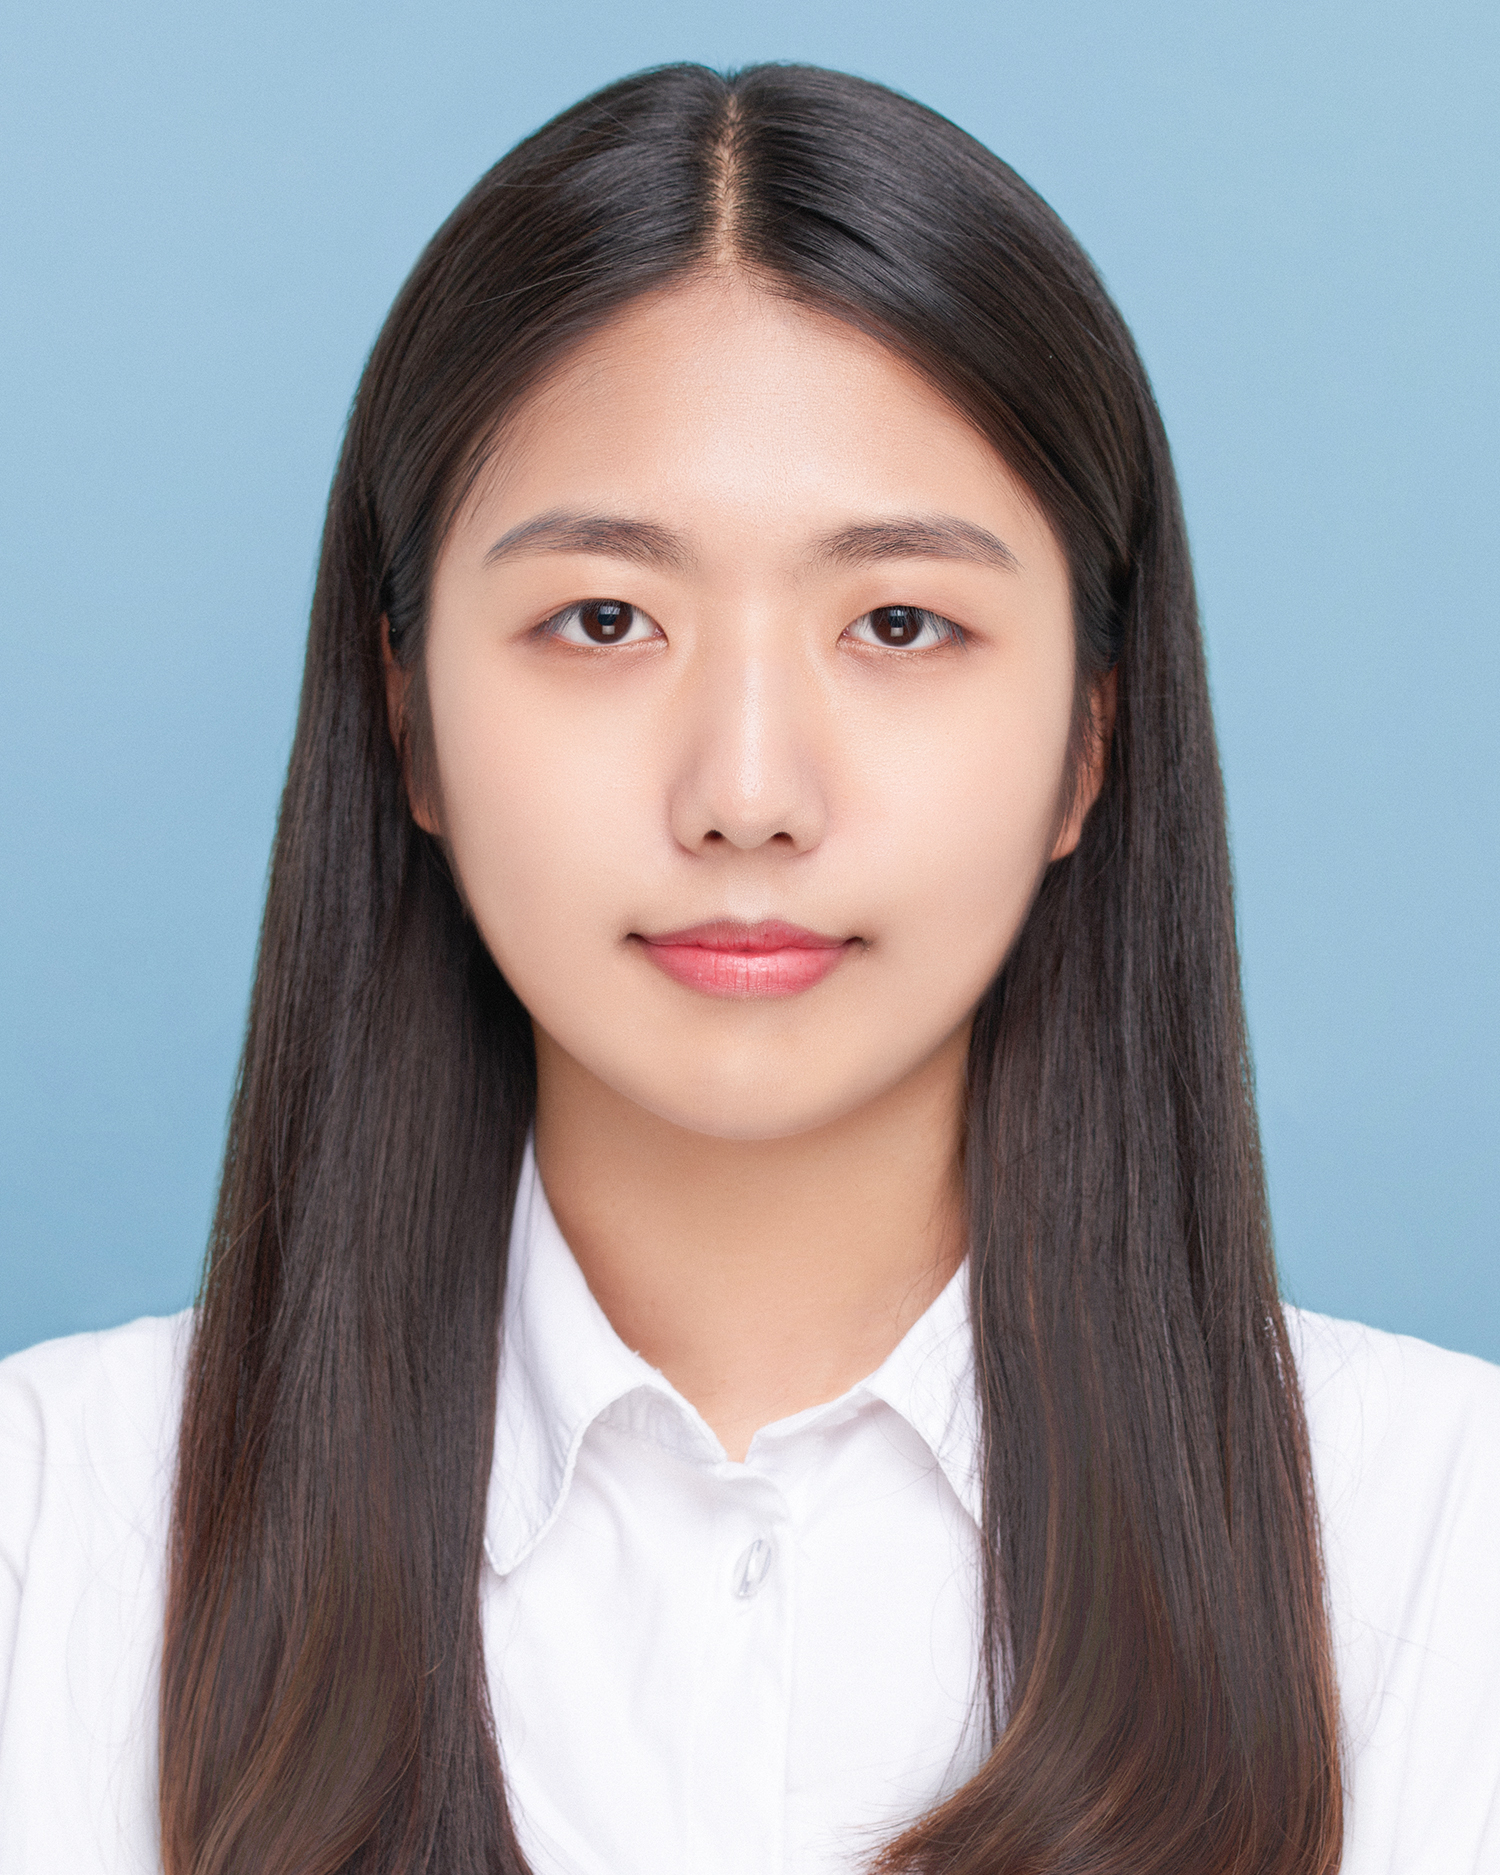
\includegraphics[width=2.2cm,clip]{증명사진.jpg}
}
\parbox{\dimexpr\linewidth-2.8cm\relax}{
\begin{tabularx}{\linewidth}{L r} \\
  \textbf{\Large \name} & {}\\
  {Department of Electrical Engineering} & {\raisebox{0.0\height}{\footnotesize \faPhone}\ \phone}\\
  \course &  \href{mailto:\emaila}{\raisebox{0.0\height}{\footnotesize \faEnvelope}\ {\emaila}} \\
  {Pohang University of Science and Technology (POSTECH)} &  \href{https://sites.google.com/view/pictuslab}{\raisebox{0.0\height}{\footnotesize \faGlobe}\ {PICTUS Lab}} \\
  {77 Cheongam-Ro, Nam-Gu, Pohang, Gyeongbuk 37673, Republic of Korea} & \href{https://www.linkedin.com/in/mun-jung-cho-a92898301}{\raisebox{0.0\height}{\footnotesize \faLinkedin}\ {LinkedIn Profile}}
\end{tabularx}
}
% \parbox{3.0cm}{%
% \flushright \includegraphics[width=2cm,clip]{nitp_logo.png}
% }

%-----------Technical skills-----------------
\section{\textbf{Research Interests}}
 \begin{itemize}[leftmargin=0.05in, label={}]
    \small{\item{
     \textbf{Power Management ICs} \\
        \hspace{0.05in} - Inductive Switching DC-DC Converter: Buck, Boost, Buck-Boost, SIMO Converter \\
        \hspace{0.05in} - Switched Capacitor Converter \\
        \hspace{0.05in} - LDO Regulator: Analog/Digital \\
     \textbf{LED Drivers} \\
     \textbf{Energy Harvesting Circuits} \\
     \textbf{Integrated Circuit Design}{: Analog, Digital, Mixed} \\
    }}
 \end{itemize}
 \vspace{-16pt}



%-----------EDUCATION-----------
\section{\textbf{Education}}
  \resumeSubHeadingListStart
    \resumeSubheading
      { Pohang University of Science and Technology (POSTECH)}{Advisor : Se-Un Shin}
      {Combined M.S/Ph.D. Program in Department of Electrical Engineering}{Sep. 2023 - Present}
    \resumeSubheading
      { Ulsan National Institute of Science and Technology (UNIST)}{Advisor : Se-Un Shin}
      {B.S. in Department of Electronic Engineering}{Feb. 2019 - Feb. 2023}
  \resumeSubHeadingListEnd
\vspace{-5.5mm}
%

%-----------PROJECTS-----------------
%\section{\textbf{Research Projects}}
%\resumeSubHeadingListStart

%    \resumeProject
%      {Project Name} %Project Name
%      {Project description(Your input in the project)} %Project Name, Location Name
%      {Event dates} %Event Dates

%      \resumeItemListStart
%        \item {Tools \& technologies used: xxx,xxx}
%        \item {More description on the project(The output you achieved by working on the project)}
%    \resumeItemListEnd
%    \vspace{-2mm}
    
%    \resumeProject
%      {Project Name} %Project Name
%      {Project description(Your input in the project)} %Project Name, Location Name
%      {Event dates} %Event Dates

%      \resumeItemListStart
%        \item {Tools \& technologies used: xxx,xxx}
%        \item {More description on the project(The output you achieved by working on the project)}
%    \resumeItemListEnd
%    \vspace{-2mm}
    
      
%  \resumeSubHeadingListEnd
%\vspace{-5.5mm}

%-----------Publications-----------------
\section{\textbf{Publications}}
 \begin{itemize}[leftmargin=0.05in, label={}]
    \small{\item{
     \textbf{International} \\
        - Yeon-Woo Jeong, Seung-Ju Lee, Jong-Hun Kim, \textbf{\underline{Mun-Jung Cho}}, Hwa-Soo Kim, Se-Un Shin, “A Scalable N-Step Equal Split SSHI Piezoelectric Enegry Harvesting Circuit Achieving 1170\% Power Extraction Improvement and 22nA Quiescent Current with a 1uH-to-10uH Low Q Inductor” 2023 IEEE International Solid-State Circuits Conference (ISSCC), Feb. 2023. \\
        \vspace{2mm}
        - Seung-Ju Lee, Yeon-Woo Jeong, \textbf{\underline{Mun-Jung Cho}}, Jong-Hun Kim, Hwa-Soo Kim, Jun-Suk Bang, Se-Un Shin, “A 95.3\% 5V-to-32V Wide Range 3-Level Current Mode Boost Converter with Fully State-based Phase Selection Achieving Simultaneous High-Speed VCF Balancing and Smooth Transition” 2023 IEEE International Solid-State Circuits Conference (ISSCC), Feb. 2023. \\
        \vspace{2mm}
     \textbf{Domestic} \\
        - \textbf{\underline{Mun-Jung Cho}}, Se-Un Shin, “Frequency Analysis of Conventional And 3-Level Buck Converter” IDEC Congress Chip Design Contest (CDC), July. 2024. \\
        \vspace{2mm}
        - \textbf{\underline{Mun-Jung Cho}}, Se-Un Shin, “Frequency Analysis of Conventional And 3-Level Buck Converter” Annual Conference of ISE, Dec. 2023. \\
        \vspace{2mm}
        - \textbf{\underline{Mun-Jung Cho}}, Seung-Ju Lee, Jong-Hun Kim, Se-Un Shin, “A High-Efficiency Du al Path Buck-Boost Converter with Wide Input Range” 2023 Korean Conference on Semiconductors (KCS), Feb. 2023. \\
        \vspace{2mm}
        - \textbf{\underline{Mun-Jung Cho}}, Se-Un Shin, “A High-Efficiency Dual Path Buck-Boost Converter with Wide Input Range” Annual Conference of ISE, Dec. 2022. \\
        \vspace{2mm}
        - \textbf{\underline{Mun-Jung Cho}}, Jong-Hun Kim, Se-Un Shin, “Design of Ladder Charge Pump with Active Gate Driving” Annual Conference of ISE, Dec. 2022. \\

    }}
 \end{itemize}
 \vspace{-16pt}


%-----------Patents-----------------
%\section{\textbf{Patents}}
%\vspace{-0.4mm}
%\resumeSubHeadingListStart
%\resumePOR{Achievement } % Award
%    {description} % Event
%    {Event dates} %Event Year
    
%\resumePOR{Achievement } % Award
%    {description} % Event
%    {Event dates} %Event Year
%\resumeSubHeadingListEnd
%\vspace{-5mm}
%\setlength{\footskip}{4.08003pt}

%-----------Honors-----------------
\section{\textbf{Honors}} %장학금
\vspace{-0.4mm}
\resumeSubHeadingListStart

\resumePOR{ 2024 Master's Student Research Scholarship } % Award
    {by the National Research Foundation} % Event
    {July, 2024 - Present} %Event Year

\resumeSubHeadingListEnd
\vspace{-5mm}
\setlength{\footskip}{4.08003pt}

%-----------EXPERIENCE-----------------
\section{\textbf{Experience}}
  \resumeSubHeadingListStart
    \resumeSubheading
      { Undergraduated Research Intern}{Advisor : Se-Un Shin}
      {Power and Integrated Circuit Technology for Universal Systems (PICTUS)}{July. 2021 - Aug. 2023}
      \vspace{-2.0mm}
      \resumeItemListStart
    \resumeItemListEnd
    
    \vspace{-3.0mm}
    
%    \resumeSubheading
%      {Company Name}{City}
%      {Your Role}{Event dates}
%      \vspace{-2.0mm}
%      \resumeItemListStart
%    \item {Work description line 1}
%    \item {Work description line 2}
%    \resumeItemListEnd
      
  \resumeSubHeadingListEnd
\vspace{-5mm}

%-----------Positions of Responsibility-----------------
%\section{\textbf{Positions of Responsibility}}
%\vspace{-0.4mm}
%\resumeSubHeadingListStart
%\resumePOR{Position, } % Position
%    {Club or Event} %Club,Event
%    {Position tenure} %Tenure Period
%\resumePOR{Position, } % Position
%    {Club or Event} %Club,Event
%    {Position tenure} %Tenure Period
%\resumeSubHeadingListEnd
%\vspace{-5mm}

%-----------Awards-----------------
%\section{\textbf{Awards}}
%\vspace{-0.4mm}
%\resumeSubHeadingListStart
%\resumePOR{Achievement } % Award
%    {description} % Event
%    {Event dates} %Event Year
    
%\resumePOR{Achievement } % Award
%    {description} % Event
%    {Event dates} %Event Year
%\resumeSubHeadingListEnd
%\vspace{-5mm}
%\setlength{\footskip}{4.08003pt}

\afterpage{
    \newgeometry{left=1.4cm, top=1.4cm, right=1.2cm, bottom=1.4cm}

%-----------Technical skills-----------------
\section{\textbf{Technical Skills}}
 \begin{itemize}[leftmargin=0.05in, label={}]
    \small{\item{
     \textbf{Simulator} \\
        \hspace{0.05in} - Cadence Virtuoso : Spectre, Calibre, Finesim \\
        \hspace{0.05in} - Synopsis : DC, ICC, StarRC for AutoPnR \\
        \hspace{0.05in} - Silvaco : SmartSpice \\
        \hspace{0.05in} - Powersim (PSIM) \\
        \hspace{0.05in} - SIMetrix/SIMPLIS \\
        \hspace{0.05in} - PSpice, LTSpice \\
     \textbf{PCB Design} \\
        \hspace{0.05in} - OrCAD \\
        \hspace{0.05in} - KiCAD \\
        \hspace{0.05in} - PADS Logic \\
    }}
 \end{itemize}
 \vspace{-16pt}


%-------------------------------------------
\end{document}
